\documentclass[fontsize=12pt,paper=a4,twoside]{scrartcl}
\usepackage{longtable} 
\usepackage{graphicx}
% SWP-Präambel
% C 2003-2017 Sebastian Offermann, Rainer Koschke, Karsten Hölscher
% In Zeilen 40 und 41 sind jeweils die aktuellen Daten einzutragen

\usepackage[utf8]{inputenc}     % Kodierung der Tex-Datei
\usepackage[T1]{fontenc}        % Korrekte Ausgabe von Sonderzeichen (Umlaute)
\usepackage[ngerman]{babel}     % Deutsche Einstellungen [ab \begin{document}]

\usepackage{bibgerm}            % Bibliographie
\usepackage{fancyhdr}           % obere Seitenränder gestalten
\usepackage{float}              % Floats Objekte mit [H] festsetzen
\usepackage{graphicx}           % Graphiken als jpg, png etc. einbinden
\usepackage{moreverb}           % zusätzliche verbatim-Umgebungen
\usepackage{pdflscape}          % PDF-Support für landscape
\usepackage[final]{pdfpages}    % Externe PDFs einbinden
\usepackage{stmaryrd}           % zusätzliche Symbole
\usepackage{supertabular}       % Tabellen über Seitenränder hinaus
\usepackage{tabularx}           % Tabellen mit vorgegebener Breite
\usepackage{url}                % setzt URLs schön mit \url{http://bla.laber.com/~mypage}

%%% Die Reihenfolge der folgenden Pakete muss beibehalten werden:
%%% varioref, hyperref, cleveref, bookmark
% Verweise innerhalb des Dokuments schick mit " ... auf Seite ... "
% automatisch versehen. Dazu \vref{labelname} benutzen
\usepackage[ngerman]{varioref}  % [vor hyperref für korrekte Verweise]
\usepackage[colorlinks=true, pdfstartview=FitV, linkcolor=blue,
            citecolor=blue, urlcolor=blue, hyperfigures=true,
            pdftex=true]{hyperref} % [vor bookmark wegen der Optionen]
\usepackage[ngerman]{cleveref}
\usepackage{bookmark}

\hyphenation{Arbeits-paket}     % Trennungsregeln

%%% Definitionen
\newcommand{\grad}{\ensuremath{^{\circ}} }
\renewcommand{\strut}{\vrule width 0pt height5mm depth2mm}
\newcommand{\gq}[1]{\glqq{}#1\grqq{}}

%%% Semesterkonstanten
\newboolean{langversion} %Deklaration
\setboolean{langversion}{true} %Zuweisung ist 'false' für Blockkurs
\newcommand{\jahr}[1]{2020} %2017/2018

% erstes Argument: SWP-2, zweites SWP-1
\newcommand{\highlight}[1]{\textcolor{blue}{\textbf{#1}}}
\newcommand{\variante}[2]{\ifthenelse{\boolean{langversion}}{#1}{#2}}
\newcommand{\nurlangversion}[0]%
    {\variante{\highlight{}}%Muss in SWP-2 ausgefüllt werden}}%
              {\highlight{Entfällt in SWP-1}}}
\newcommand{\swp}[0]{Software-Projekt \variante{2}{1}}
\newcommand{\semester}[0]{SoSe \jahr}

%%% Formatierungsanpassungen
% Damit Latex nicht zu lange Zeilen produziert:
\sloppy
%Uneinheitlicher unterer Seitenrand:
%\raggedbottom

% Kein Erstzeileneinzug beim Absatzanfang
% Sieht aber nur gut aus, wenn man zwischen Absätzen viel Platz einbaut
\setlength{\parindent}{0ex}

% Abstand zwischen zwei Absätzen
\setlength{\parskip}{1ex}

% Seitenränder für Korrekturen verändern
\addtolength{\evensidemargin}{-1cm}
\addtolength{\oddsidemargin}{1cm}

\bibliographystyle{gerapali}

% 1. Parameter: Euer/Eure TutorIn, z. B. {Kim Harrison}
% 2. Parameter: Abgabedatum, z. B. {05. April 2063}
% 3. Parameter: Versionsnummer, z. B. {1.1}
% 4.-9. Parameter: jeweils Name und (Uni-)Email-Adresse jedes 
%                 Gruppenmitglieds; mit einem & getrennt, z. B.
% {Robin Cowl & roco@tzi.de}
% Besteht die Gruppe aus weniger als 6 Personen, so werden die 
% übrigen Parameter leer gelassen: {}
\newcommand \swpdocument[9] {
% Lustige Header auf den Seiten
  \pagestyle{fancy}
  \setlength{\headheight}{70.55003pt}
  \fancyhead{}
  \fancyhead[LO,RE]{\swp{}\\%
                    \semester{}\\%
                    \documentTitle}
  \fancyhead[LE,RO]{Seite \thepage\\%
                    \slshape \leftmark\\%
                    \slshape \rightmark}

% Lustige Header nur auf dieser Seite (Titelseite)
  \thispagestyle{fancy}
  \fancyhead[LO,RE]{ }
  \fancyhead[LE,RO]{Universität Bremen\\%
                    FB 3 -- Informatik\\%
                    Dr. Karsten Hölscher\\%
                    TutorIn: #1}
  \fancyfoot[C]{}

% Start Titelseite
  \vspace{3cm}
  \begin{minipage}[H]{\textwidth}
    \begin{center}
      \bfseries \Large \swp{} -- \semester{}\\
      \smallskip
      \small VAK 03-BA-901.02\\
      \vspace{3cm}
    \end{center}
  \end{minipage}
  \begin{minipage}[H]{\textwidth}
    \begin{center}
      \vspace{1cm}
      \bfseries \Large \documentTitle\\
      \vfill
    \end{center}
  \end{minipage}
  \vfill
  \begin{minipage}[H]{\textwidth}
    \begin{center}
      \sffamily
      \begin{tabular}{lr}
        #4 \\
        #5 \\
        #6 \\
        #7 \\
        #8 \\
        #9 \\
      \end{tabular}
      \\[22mm]
      \itshape Abgabe: #2 --- Version #3 \\ ~
    \end{center}
  \end{minipage}
% Ende Titelseite

% Start Inhaltsverzeichnis
\newpage
  \thispagestyle{fancy}
  \fancyhead{}
  \fancyhead[LO,RE]{\swp{}\\%
                    \semester{}\\%
                    \documentTitle}
  \fancyhead[LE,RO]{Seite \thepage\\%
                    \slshape \leftmark\\~}
  \fancyfoot{}
  \renewcommand{\headrulewidth}{0.4pt}
  \tableofcontents
% Ende Inhaltsverzeichnis

% Header für alle weiteren Seiten
\newpage
  \fancyhead[LE,RO]{Seite \thepage\\%
                    \slshape \leftmark\\%
                    \slshape \rightmark}

}



%
% Und jetzt geht das Dokument los....
%
\begin{document}
\newcommand\documentTitle{Benutzerhandbuch}
 %\begin{minipage}[b]{\textwidth}
 \vspace{1mm}
 \begin{figure}[!b]
  \centering
  
\includegraphics[width=0.5\textwidth]{pics/SpaceStudioLogo.png}\\
\end{figure}

\swpdocument{Dr. Karsten Hölscher}{02. August 2020}{1.1}%
            {Clara Maria Odinius & odinius@uni-bremen.de}%
            {Habib Mergan & habib1@uni-bremen.de}%
            {Kevin Santiago Rey Rodriguez & kev\_rey@uni-bremen.de}%
            {Liam Hurwitz & hurwitz@uni-bremen.de}%
            {Mehmet Ali Baykara & baykara@uni-bremen.de}%
            {Miguel Alejandro Caceres Pedraza & mcaceres@uni-bremen.de}%

%%%%%%%%%%%%%%%%%%%%%%%%%%%%%%%%%%%%%%%%%%%%%%%%%%%%%%%%%%%%%%%%%%%%%%%%



%%%%%%%%%%%%%%%%%%%%%%%%%%%%%%%%%%%%%%%%%%%%%%%%%%%%%%%%%%%%%%%%%%%%%%%%
\section{Einführung}

Willkommen beim Spacestudio Game!\\
Dieses Benutzerhandbuch beschreibt, wie die Software bzw. das Spiel gespielt wird und dient somit als Anleitung für das Programm.
Lesen Sie sich dieses Handbuch aufmerksam durch bevor Sie die Anwendung starten, um alle Funktionalitäten des Spiels kennen zu lernen und zu verstehen.

Dieses Spiel ist nach dem Vorbild des bekannten Spiels Faster Than Light entwickelt worden, daher werden Sie viele Parallelen zwischen diesen beiden Spielen feststellen können.

%%%%%%%%%%%%%%%%%%%%%%%%%%%%%%%%%%%%%%%%%%%%%%%%%%%%%%%%%%%%%%%%%%%%%%%%
\subsection{Zweck}

Dieses Benutzerhandbuch ist im Rahmen von ReSWP 2 SoSe2020  der Gruppe SpaceStudio geschrieben.
Der Zweck dieses Handbuches besteht darin, eine Anleitung zu dem entwickleten Spiel bereit zu stellen, damit sowohl das Spiel selbst, als auch unsere Gedanken und Ideen bezüglich der vielen einzelnen Elemente nachvollzogen werden können.

%%%%%%%%%%%%%%%%%%%%%%%%%%%%%%%%%%%%%%%%%%%%%%%%%%%%%%%%%%%%%%%%%%%%%%%%

\section{Installation}
In diesem Abschnitt wird beschieben, wie das Programm installiert wird und entsprechende Systemvoraussetzungen aufgelistet.

\subsection{Systemvoraussetzungen}
1. Java 11 oder höher \\
2. Windows 10, macOS, Linux \\
3. Gradle 5.2 oder höher \\
4. Spring Boot 2.0.3.RELEASE \\
5.  Spring Framework 5.0.7.RELEASE or höher. \\
6. 1920X1080 Auflösung
 

\subsection{Installationsschritte}
Folgende  Schritte sind für Installation benötigt. \\
1. Nach dem Sie alle benötigte tools, die in Systemvoraussetzungen aufgelistet wurden, installiert haben \\
2. Starten Sie der Server und warten Sie bis der Server hochfährt (ca 1 Minute)\\
3. Wenn der Server gestartet erfolreich gestartet wurde, starten Sie den Client.

 


%%%%%%%%%%%%%%%%%%%%%%%%%%%%%%%%%%%%%%%%%%%%%%%%%%%%%%%%%%%%%%%%%%%%%%%%

\section{Start}

Startet der Client, dann zeigt sich sich der Registrierungs und Login Screen.
Registrieren Sie sich über die Eingabefelder auf der rechten Seite. Dazu wählen Sie einen Benutzernamen und Passwort, welches zwei Mal wiederholt eingegeben werden muss, um fehlerhafte Eingaben zu vermeiden.
War die Registrierung erfolgreich, bekommen Sie die Rückmeldung Successfully created, anderen falls erscheint Password does not match oder sofern der Benutzname schon vergeben wurde Name already
registered, try another one.\\
Nach erfolgreicher Registrierung geben Sie ihre Benutzernamen und Passwort in die linken Eingabefelder ein, ist auch der Login erfolgreich erscheint die Rückmeldung login... .\\

Hinweis: Gib es Probleme mit der Registrierung, empfehlen wir den Server erneut zu starten.

\subsection{Anmeldung}
\begin{figure}[htp]
\centering
	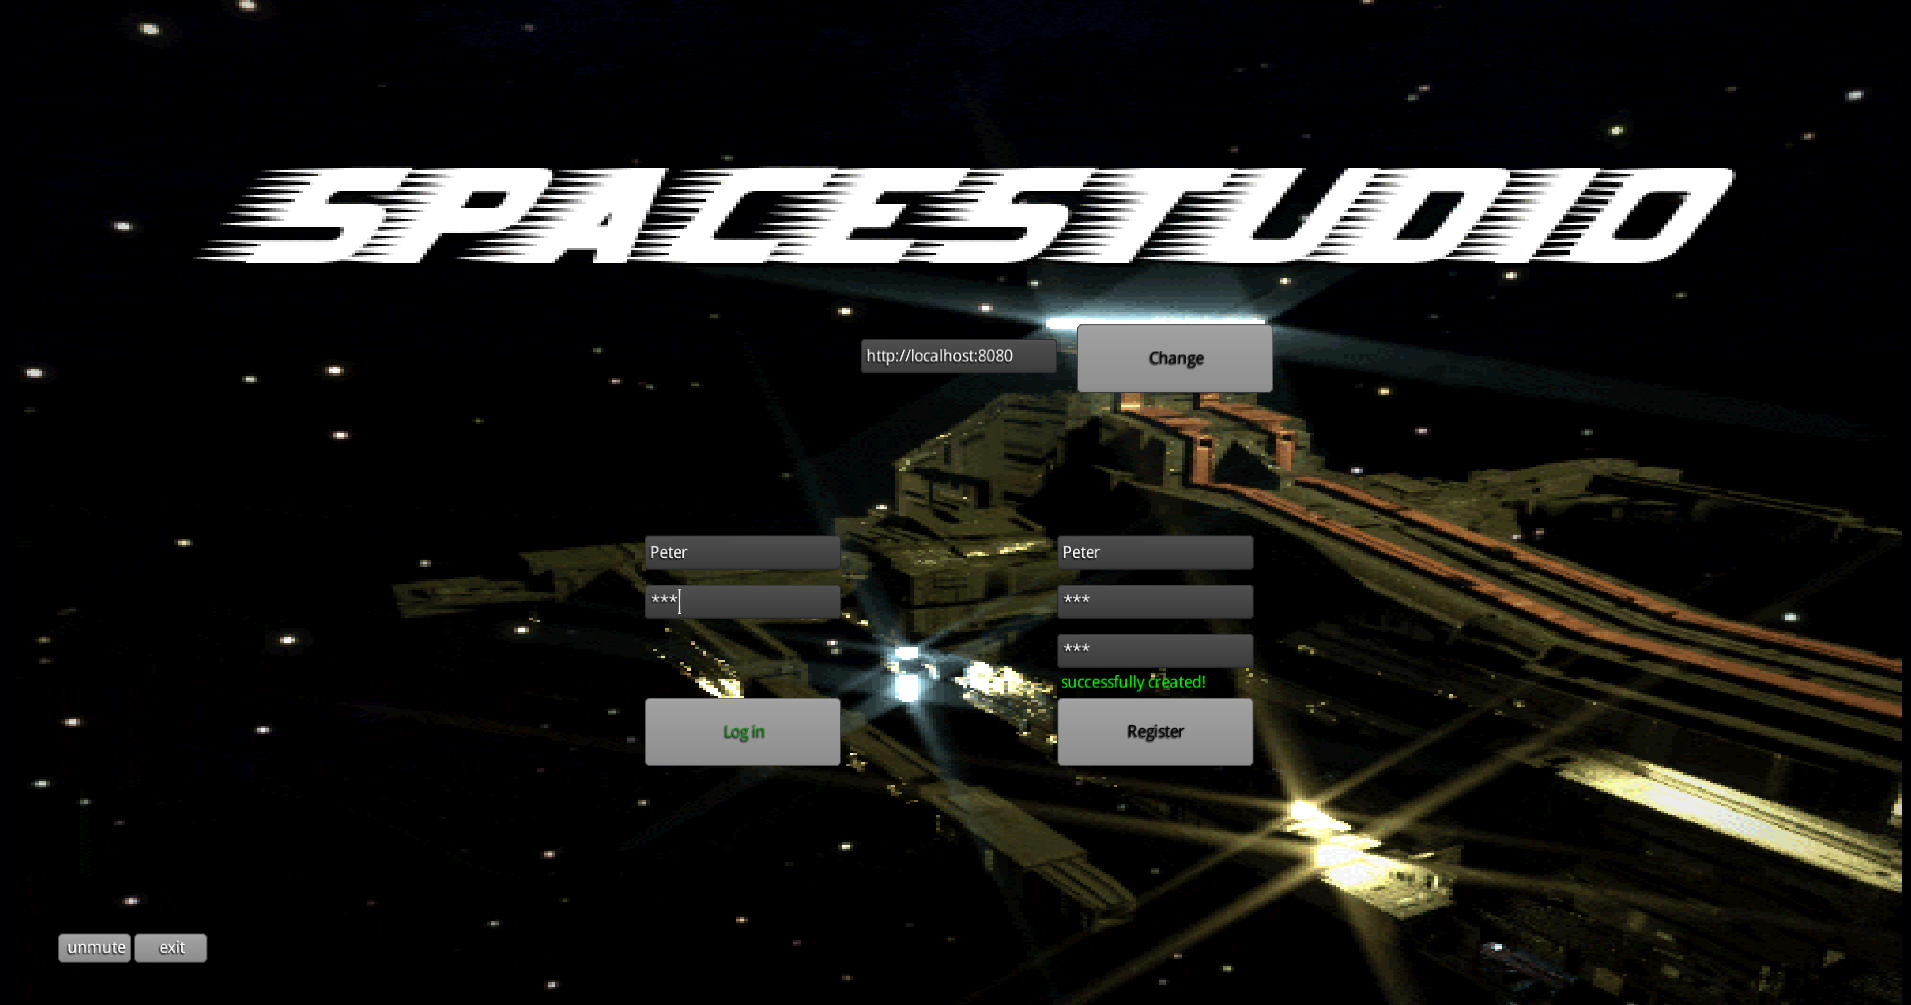
\includegraphics[width=1.00\linewidth]{pics/StartScreen01.png}
	\caption{Anmeldung: Registrierung und Login}
	\label{fig1}
\end{figure}

Der Start Screenerstellt erzeugt ein Profil mit welchem sich der Benutzer jeder Zeit wieder beim Spiel einloggen kann, um auf die gespeicherten Spieldaten wieder zurückgreifen zu können. \\
Darüber hinaus besteht die Möglichkeit eine Netwerkadresse einzugeben, falls zu einem Späteren Zeitpunkt der Multiplayer-Modus gewählt wird, dazu mehr im Kapitel Multiplayer-Modus.\\
In der unteren linken Ecke des Fensters befinden sich die zwei Button mute und exit. Über den Mute-Button lässt sich die Hintergrundmusik an- und ausschalten. 
Über den Exit-Button kann das Spiel ohne weiteres beendet werden.

\newpage

%%%%%%%%%%%%%%%%%%%%%%%%%%%%%%%%%%%%%%%%%%%%%%%%%%%%%%%%%%%%%%%%%%%%%%%%
\subsection{Menu}

Nach dem Registrierungs und Login Screen folgt das Menü:\\
Zu sehen sind die drei Button New Game, Options und Exit. Sofern vorher schon ein Spiel begonnen wurde, erscheint auch der Button Continue.\\

\begin{figure}[htp]
	\centering
	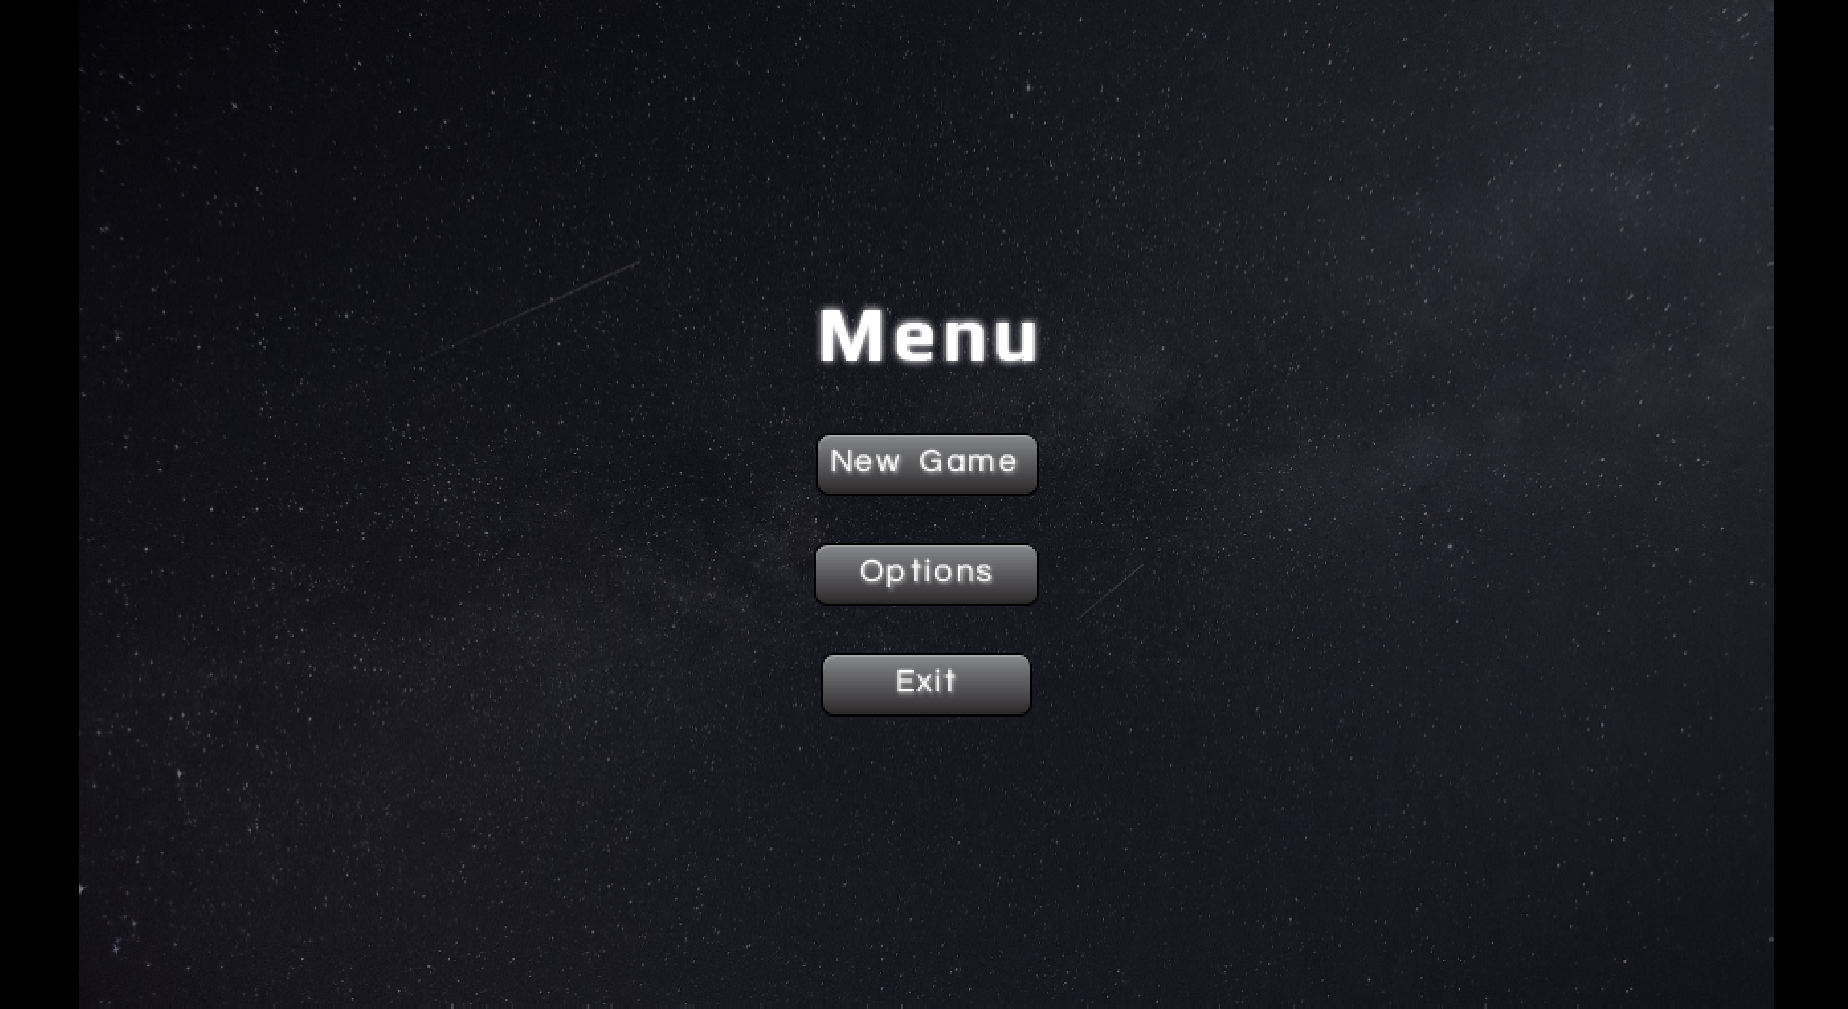
\includegraphics[width=1.00\linewidth]{pics/menuscreen.png}
	\caption{Menu}
	\label{fig1}

\end{figure}

Über New Game kann ein neues Spiel begonnen werden. \\
Continue ermöglicht es, ein zuvor begonnenes Spiel weiter zu Spielen, da jeder Spielstand gespeichert werden kann.\\
Options ist derzeit nicht verfügbar und kann für persönliche Anpassungen implementiert werden. \\
Exit beendet das Programm umgehend, ohne zur Startseite zurück zu gelangen.\\

\newpage
%%%%%%%%%%%%%%%%%%%%%%%%%%%%%%%%%%%%%%%%%%%%%%%%%%%%%%%%%%%%%%%%%%%%%%%%
\subsection{New Game}

Sofern im Menu Screen new Game ausgewählt wurde, folgt der New Game Screen.\\
Hier ergeben sich die Möglichkeiten ein Single Player Spiel oder ein Multiplayerspiel zu starten, oder aber zurück zum Menü zu gelangen.\\

\begin{figure}[htp]
	\centering
	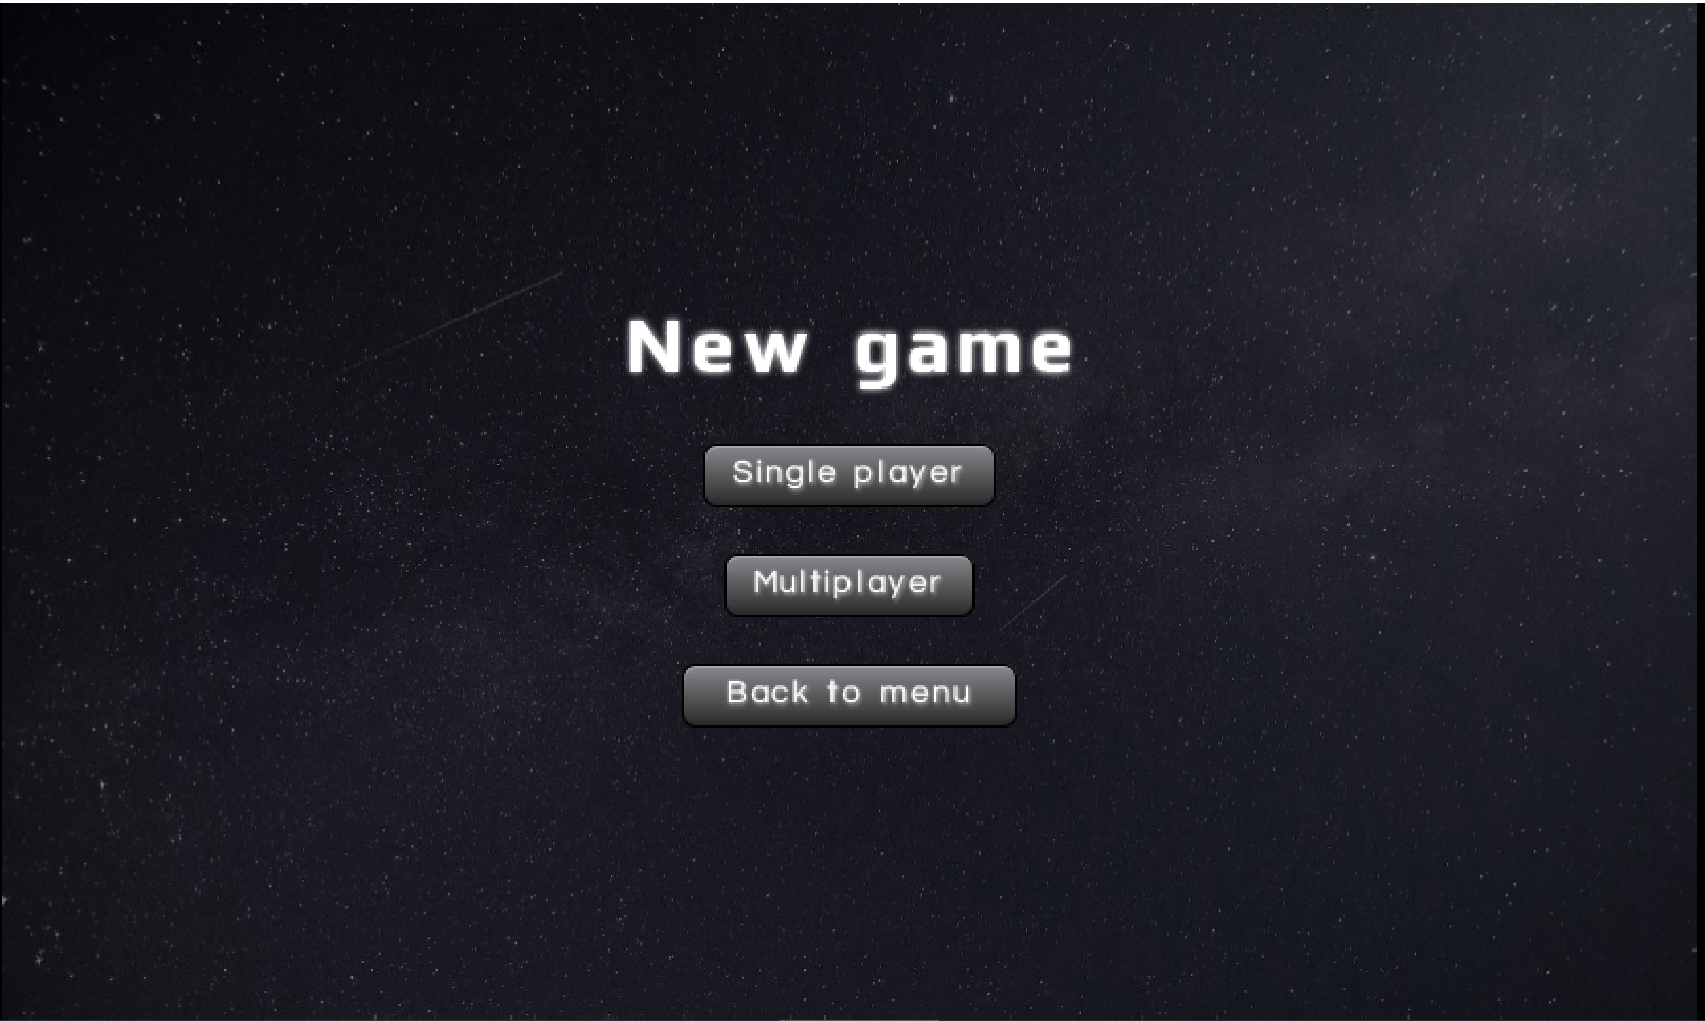
\includegraphics[width=1.00\linewidth]{pics/gamemodescreen.png}
	\caption{Spielmodus}
	\label{fig1}
\end{figure}

\subsection{Single Player}

Hier sehen Sie den Screen, der erscheint, wenn Sie Single Player im New Game Screen gewählt haben:\\
Mittig werden die Raumschiffe angezeigt, die in dem Universum existieren, derzeit verfügt der Spieler aber nur über die Möglichkeit mit dem blauen Schiff zu spielen.\\
Über previous und next lassen sich die Raumschiffe der Zukunft anzeigen. Über den Button Show rooms unterhalb des Raumschiffs, erscheinen die Sektionen, sowie dessen Ausstattung
und Besatzung.

\begin{figure}[htp]
	\centering
	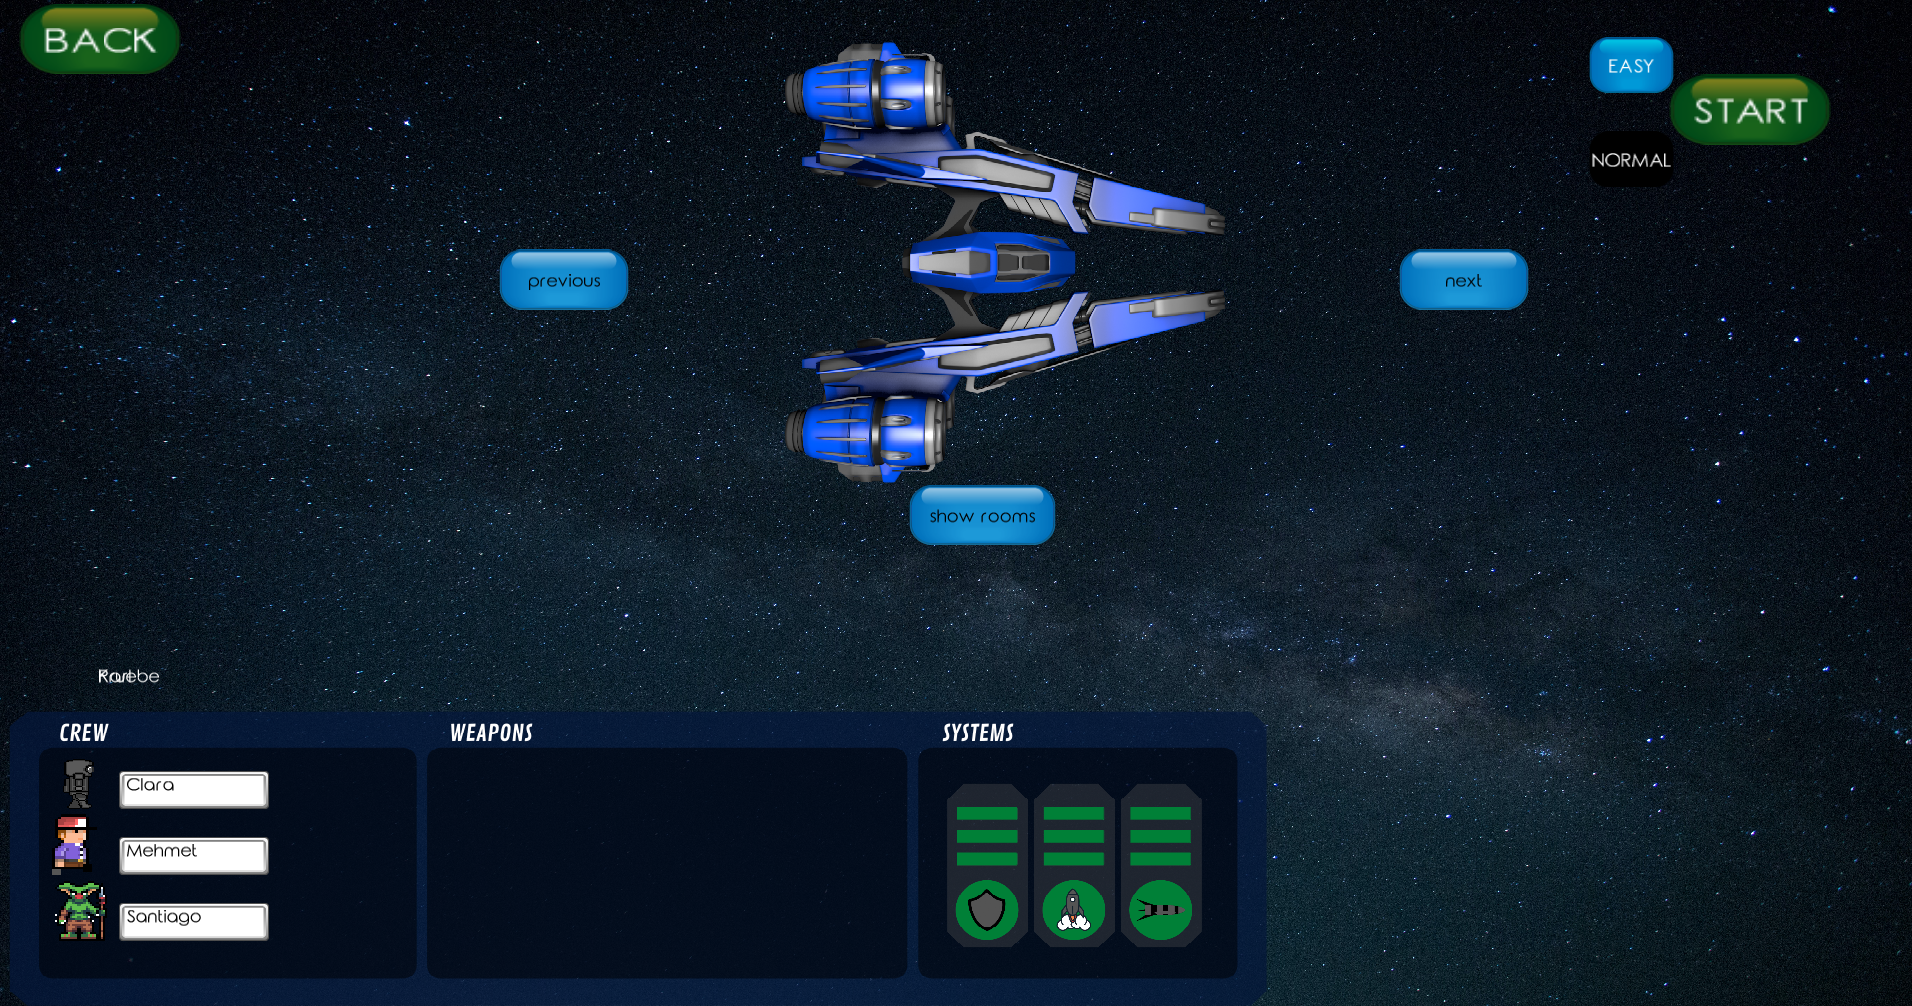
\includegraphics[width=1.00\linewidth]{pics/SinglePlayer01.png}
	\caption{Single Player}
	\label{fig1}
\end{figure}

Die Anzeige am unteren Bildschirmrand zeigt die zugehörigen Crew Member und dessen Namen, sowie über welche Systeme das Raumschiff verfügt.\\
Links neben dem Start Button kann eine weitere Auswahl zwischen Easy und Normal getroffen werden, diese Modi entscheiden über den Schwierigkeitsgrad des Spiels.\\
Über Start beginnt das Spiel mit der Ausgefählen Spielstufe.
Der Button Back oben links in der Ecke des Fensters, leitet zurück zum New Game Screen.\\
Im Single Player Modus werden die Gegner, auf die der Spiele im laufe des Spiels trifft durch eine KI realisiert.

\newpage
%%%%%%%%%%%%%%%%%%%%%%%%%%%%%%%%%%%%%%%%%%%%%%%%%%%%%%%%%%%%%%%%%%%%%%%%
\subsection{Multiplayer}

Hier sehen Sie den Screen, der erscheint, wenn Sie  Multiplayer im New Game Screen gewählt haben:\\
Dieser Screen unterscheidet sich in sofern vom Singlaplayer Screen, dass eine zusätzliche Anzeige erscheint, der Sie entnehmen können, wie viele weitere Spieler online sind.\\
Damit weiter Spieler erscheinen müssen diese im Login Screen die selber Netzwerkadresse angegeben haben/ auf dem gleichen Server angemeldet sein und ebenfalls den Multiplayer Modus augewählt haben.\\
Außerdem entfällt die Wahl der Spielstufe, da der Gegner nun nicht mehr durch den Computer ersetzt werden muss.

\begin{figure}[htp]
	\centering
	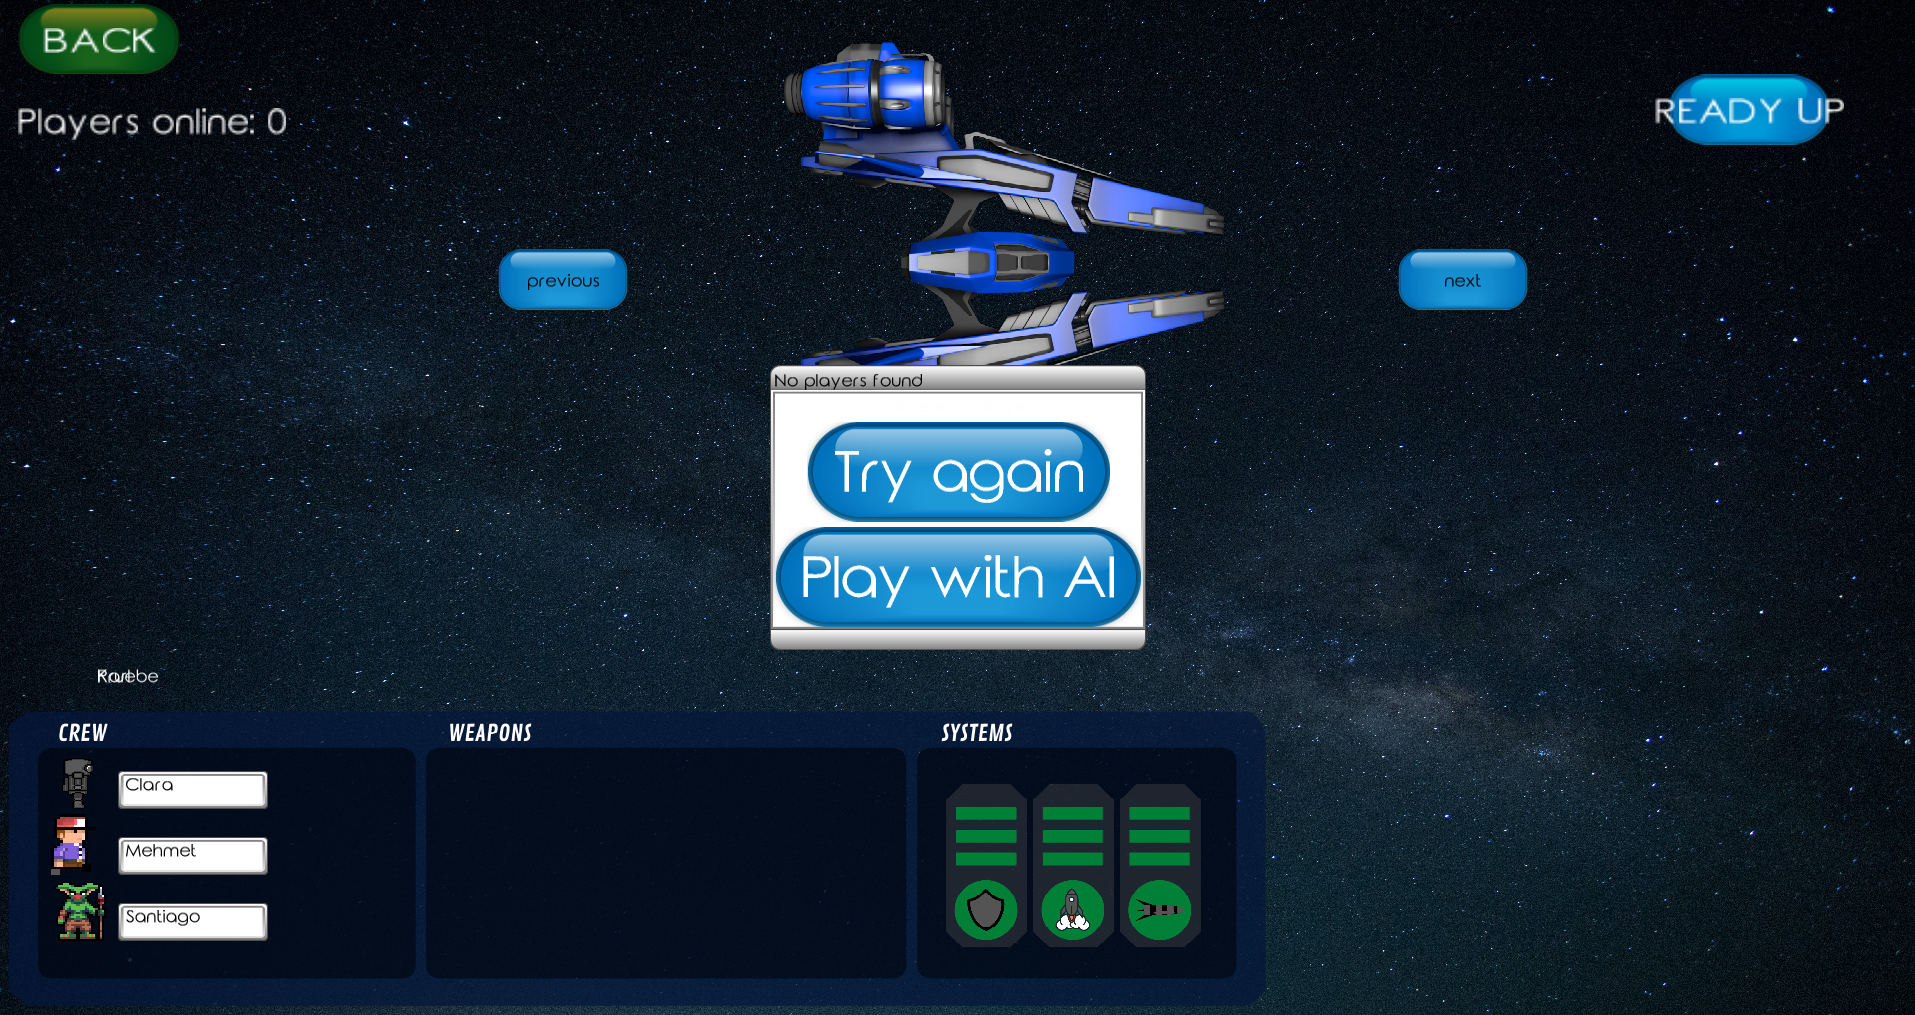
\includegraphics[width=1.00\linewidth]{pics/MultiPlayer01.png}
	\caption{Single Player}
	\label{fig1}
\end{figure}

Für den Fall, dass keine weiteren Spieler gefunden werden, erscheint ein Pop up Fenster das die Möglichkeiten bietet, über Try again erneut nach anderen Spielern zu suchen
oder sich über Play with AI doch zu einem Spiel im Single Player Modus umzuentscheiden.\\
 
\newpage
%%%%%%%%%%%%%%%%%%%%%%%%%%%%%%%%%%%%%%%%%%%%%%%%%%%%%%%%%%%%%%%%%%%%%%%%
\section{Spielstufen Easy und Normal}


Beschreibung der Spielmodus.
%%%%%%%%%%%%%%%%%%%%%%%%%%%%%%%%%%%%%%%%%%%%%%%%%%%%%%%%%%%%%%%%%%%%%%%%
\subsection{Map}
Beschreibung der Spielmodus.

%%%%%%%%%%%%%%%%%%%%%%%%%%%%%%%%%%%%%%%%%%%%%%%%%%%%%%%%%%%%%%%%%%%%%%%%
\section{Eigentliches Spiel}
Beschreibung der Kamfscreen.
%%%%%%%%%%%%%%%%%%%%%%%%%%%%%%%%%%%%%%%%%%%%%%%%%%%%%%%%%%%%%%%%%%%%%%%%
\subsection{Spiel Verlauf}
Beschreibung der Spielmodus.
%%%%%%%%%%%%%%%%%%%%%%%%%%%%%%%%%%%%%%%%%%%%%%%%%%%%%%%%%%%%%%%%%%%%%%%%

\subsection{Spiel Unterbrechung}
Beschreibung der Unterbrechung des Spiels und fortsetzen.
%%%%%%%%%%%%%%%%%%%%%%%%%%%%%%%%%%%%%%%%%%%%%%%%%%%%%%%%%%%%%%%%%%%%%%%%


\subsection{Spiel Wiedergeben}
Spielzüge detaliert wiedergeben
\end{document}

%%% Local Variables: 
%%% mode: latex
%%% mode: reftex
%%% mode: flyspell
%%% ispell-local-dictionary: "de_DE"
%%% TeX-master: t
%%% End: 
